
\chapter{Implementation}\label{section:implementation}

\section{Overview of Important Class Diagrams}

As stated in section~\ref{section:aims}, this project extends from SICSA project which uses only publications as expertise evidence.
The aim of this project is to integrate funded projects with publications to improve the performance of the retrieval system.
Figure~\ref{fig:classDiagram1} shows the relationship between Candidate (Expert), Project, Publication and University classes. Each component in the figure
shows only important attributes and methods. The Candidate class represents an expert who lectures at a university and has a set of publications and projects.
\begin{figure}
\centering
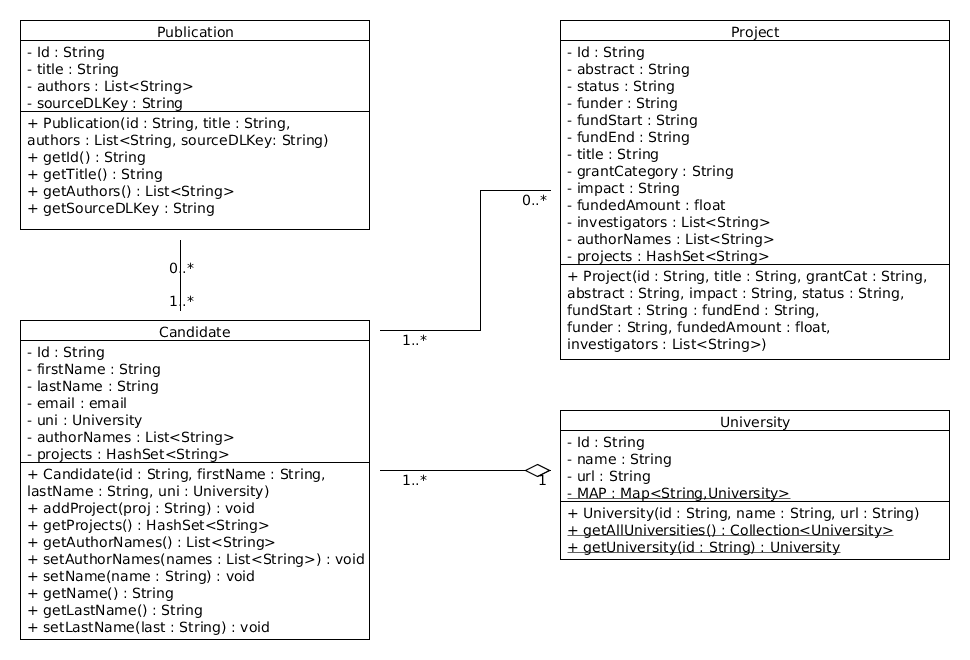
\includegraphics[scale=0.4]{./figures/classDiagram1.png}
\caption{Class Diagram} \label{fig:classDiagram1} 
\end{figure}

As stated in section ~\ref{section:goodexpert}, the features extracted from funded projects and publications of each expert will be used in Learning to Rank
to improve the retrieval performance of the system. But before we get to Learning to Rank, first of all, we need to understand
AcademTechQuerying Class and RetrievedResults Class which are components used in retrieving results with respect to a query. 
\begin{figure}
\centering
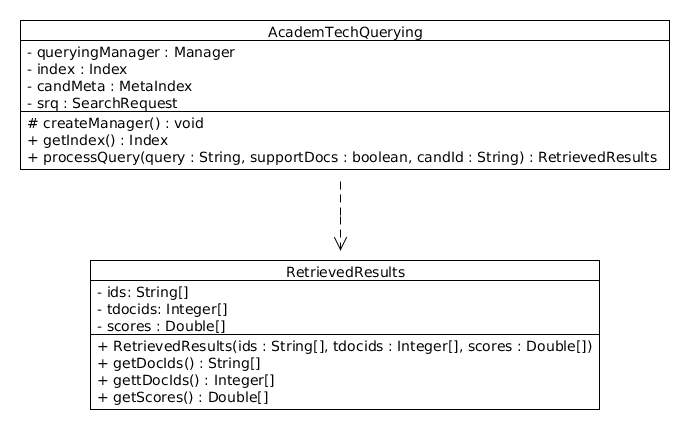
\includegraphics[scale=0.4]{./figures/AcademTechQuerying.png}
\caption{AcademTechQuerying Class and RetrievedResults Class} \label{fig:AcademTechQuerying} 
\end{figure}

Figure~\ref{fig:AcademTechQuerying} shows class diagrams of AcademTechQuerying and RetrievedResults. As stated in section~\ref{section:terrier},
the search engine platform used in this project is Terrier. It handles indexing and retrieval processes discussed in section~\ref{section:IRarchitecture}.
The AcademTechQuerying Class makes use of 2 Terrier components as follows:  
\begin{itemize}
 \item \textit{queryingManager} of type Manager, responsible for handling/co-ordinating the main high-level operations of a query.
 \item \textit{srq} of type SearchRequest, responsible for retrieving search result from Manager.
\end{itemize}
The most important method of AcademTechQuerying is processQuery(). It returns RetrievedResults component. This method takes a query string, supportDocs and candId as arguments. The first argument tells
the system that a query is used to retrieve the result, the second and third arguments are used in case the system wants documents associated to a candidate 
with respect to a query.

The RetrievedResults Class has 3 attributes as follows:
\begin{itemize}
 \item ids, an array of String, which is the ids of the documents(in this case, ids of experts) retrieved by the system.
 \item tdocids, an array of Integer, which is the ids used by Terrier
 \item scores, an array of Double, which is the scores of each document retrieved by the system.
\end{itemize}

\section{Data Extraction}
\begin{figure}
\centering
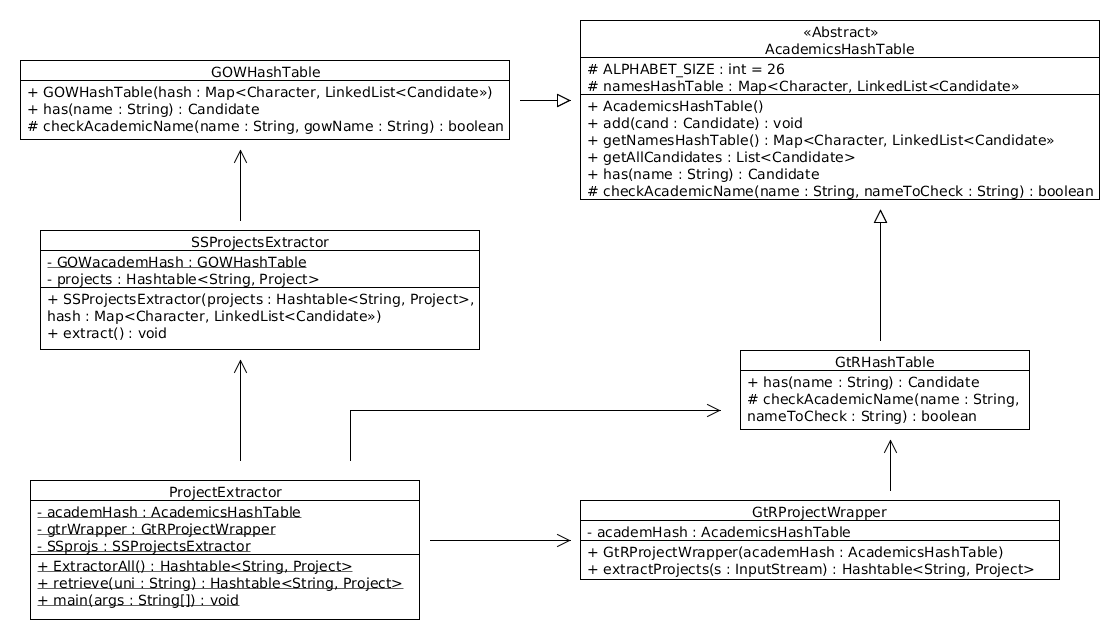
\includegraphics[scale=0.35]{./figures/projectsExtraction.png}
\caption{Projects Extraction Class Diagrams} \label{fig:projectsExtraction} 
\end{figure}
In section~\ref{section:aims}, it was stated that funded projects are obtained from Grant on the Web~\cite{gow} and Research Councils UK~\cite{gtr}.
This section shows classes used to extract funded projects from each source and gives statistics regarding the number of funded projects from each source.
Figure~\ref{fig:projectsExtraction} shows class diagram related to projects extraction task.
\paragraph{AcademicsHashTable} is an abstract class which makes use of HashMap data structure, Map<Character, LinkedList<Candidate>>, for efficient look up when matching candidate to our
known candidates. It is keyed by the first character of candidate's name. There are 2 abstract methods in this class: has() and checkAcademicName() methods.
Both of them are used together to check if the candidate is matched to our known candidates.
\paragraph{GtRHashTable} extends from the abstract class AcademicsHashTable. The purpose of this class is the same as AcademicsHashTable Class but
implements has() and checkAcademicName() methods which are applicable in Research Councils UK~\cite{gtr} data source.
\paragraph{GOWHashTable} extends from the abstract class AcademicsHashTable. Its purpose is similar to AcademicsHashTable Class but
has different implementations of hash() and checkAcademicName() methods to GOWHashTable's which are applicable in Grant on the Web~\cite{gow} spreadsheet data source.
\paragraph{SSProjectsExtractor} is a class that makes use of GOWHashTable Class to extract funded projects from Grant on the Web~\cite{gow} spreadsheet.
\paragraph{GtRProjectWrapper} is a class used GOWHashTable Class to extract funded projects from Research Councils UK~\cite{gtr}.
\paragraph{ProjectExtractor} is a class that makes use of SSProjectsExtractor and GtRProjectWrapper Classes to extract funded projects from both sources.

The most difficult part in extracting projects is to match the known expert's names with the expert's names in each source. This is because each source
records expert's name in different formats. For example, Prof. Joemon Jose may be recorded Jose JM in one source and Jose J in another. This is why Polymorphism~\cite{polymorphism} 
(different implementations of has() and checkAcademicName() methods between GtRHashTable and GOWHashTable) is required. However, pattern matching between
expert's names in Grant on the Web~\cite{gow} spreadsheet is still impossible as this source records in the following format: 
[lastname], [role] [the first letter of name] such as Jose, Professor JM. The problem occurs with experts, Dr. Craig Macdonald lecturing at
University of Glasgow and Prof. Catriona Macdonald lecturing at Glasgow Caledonian University
as the source records Macdonald, Dr C for the former and Macdonald, Professor C for the latter. Although, role might be used to distinguish between them but
for some experts the role is not known and there might be the situation that the role is also the same. 
Therefore, university is used as part of the matching as well.

\begin{table}
\centering
\begin{tabular}{|c|c|}
\hline \textbf{Source} & \textbf{Number of Funded Projects} \\
\hline Grant on the Web & 32 \\
\hline Research Councils UK & 337 \\
\hline   & 369 total \\ 
\hline
\end{tabular}
\caption{The number of funded projects extracted from each source} \label{table:stats}
\end{table}
Figure ~\ref{table:stats} shows the number of funded projects extracted from each source. There are 1569 known candidates in the system.

\section{Indexing}
\begin{table}
\centering
\begin{tabular}{|c|c|}
\hline Number of experts & 1569 \\
\hline Number of publications UK & 22225 \\
\hline Number of all documents   & 25311 \\ 
\hline Number of tokens (terms) & 6976895 \\
\hline
\end{tabular}
\caption{Statistics of New System} \label{table:newtstats}
\end{table}
Table~\ref{table:newtstats} shows statistics of new system after indexing.


\section{Producing a Learned Model}\label{section:producelearnedmodel}
Section ~\ref{section:learnedmodel} described general steps to producing a learned model. This section aims to discuss classes involved in producing a learned model.
As section~\ref{section:learnedmodel} suggested, the first step in producing a learned model is to generate a set of training queries. 
Then all features described in Section~\ref{section:goodexpert} for each document (expert) with respect to each training query are extracted and saved
in a file. This file in learning to rank is called LETOR file. Figure~\ref{fig:sampleletorfile} is a sample LETOR file. The lines preceded by hash key are 
ignored. They are just headers which describe features. There are 7 features as described section ~\ref{section:goodexpert}.
The numbers after a hash key indicate features id. However, the lines not preceded by hash key are learned. They represent documents (experts) with scores
of each feature attached to them. They are preceded by numbers. These numbers in learning to rank are labels which indicate the degree of relevancy.
If the label is 0, it means the expert is irrelevant with respect to a query. If it is 1, the expert is relevant. However, the label needs not be binary.
It could range from 0 to any positive number. The higher the number, the more relevant the expert is. In this project, labels range from 0 to 2 in order of 
the degree of relevancy. To the left of the label is query id and scores of each feature associated to that expert. Again, within these lines, anything after hash key is ignored.
\begin{figure}
\centering
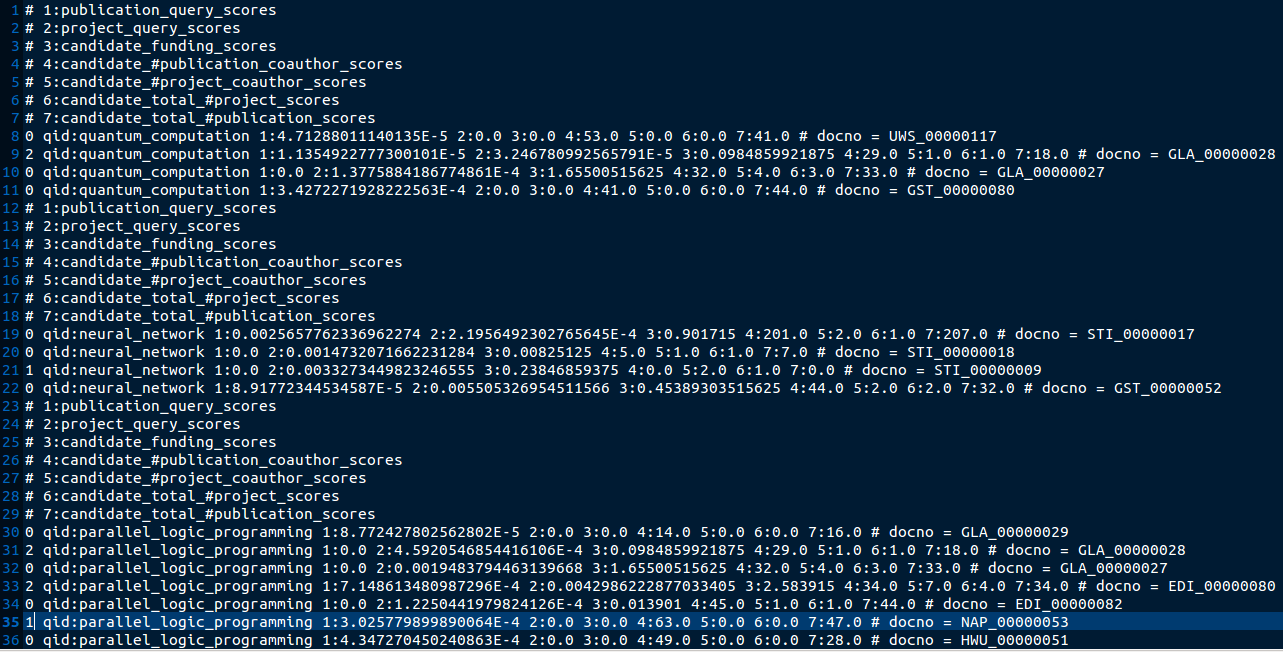
\includegraphics[scale=0.3]{./figures/sampleletorfile.png}
\caption{Sample LETOR file} \label{fig:sampleletorfile} 
\end{figure}



\begin{figure}
\centering
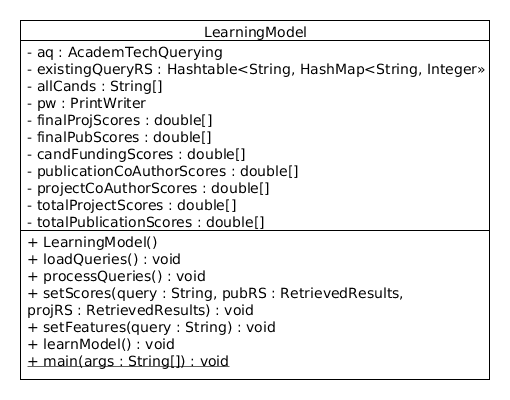
\includegraphics[scale=0.7]{./figures/learningModel.png}
\caption{Class Diagram of LearningModel} \label{fig:learningmodel} 
\end{figure}

Figure ~\ref{fig:learningmodel} shows a class diagram that is used to produce a learned model. There are 5 important methods as follows
\begin{itemize}
 \item loadQueries() is a method that loads all training queries from a file.
 \item processQuery() is a method that retrieve documents (experts) with respect to publication query and project query.
 \item setScores() is a method that performs a union between results with respect to publication query and project query as discussed in Section ~\ref{section:union}
 \item setFeatures() is a method that extracts features for each document (expert) and write into a LETOR file.
 \item learnModel() is a method that produces a learned model using RankLib~\ref{section:rankLib}.
\end{itemize}

As stated in Section ~\ref{section:rankLib}, learning to rank algorithms used in this project are AdaRank and Coordinate Ascent. The performance of each
of them will be discussed in Evaluation Section. Figure~\ref{fig:samplemodel} shows a sample model. Similar to LETOR file, lines preceded by hash key are
ignored. They are just headers which describe parameters used in the learning to rank algorithm. Knowing what each parameter does is out of the scopre of 
this project. This model is obtained using Coordinate Ascent Algorithm. The numbers before colons are features id and after colons are scores of each 
feature. Section~\ref{section:applyinglearnedmodel} will explain how learned model is applied to get optimal ranking.

\begin{figure}
\centering
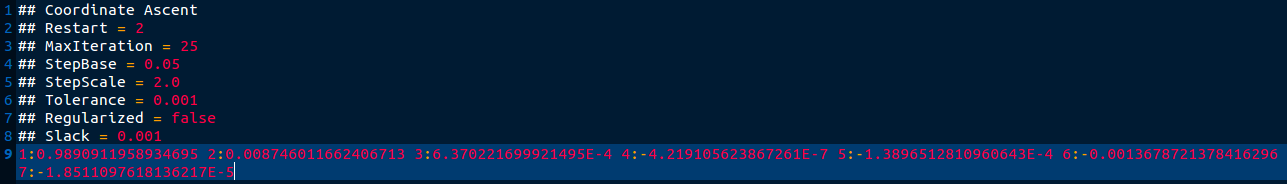
\includegraphics[scale=0.3]{./figures/samplemodel.png}
\caption{Sample Model} \label{fig:samplemodel} 
\end{figure}

\section{Applying a Learned Model}\label{section:applyinglearnedmodel}
Now that a learned model has been generated, this learned model can be applied to produce optimal ranking. Given a query,
scores of query dependent features are computed for each expert as shown in figure~\ref{fig:quering}. After that, scores of query independent feaures
of experts obtained from querying are extracted. Then for each expert, the scores of each feature are multiplied by ones in the learned model and accumulated.
Finally, the accumulated scores for each expert are sorted in descending order and experts with the high scores are ranked before those with low scores. 
This was briefly explained in section~\ref{section:learnedmodel}.



\begin{figure}
\centering
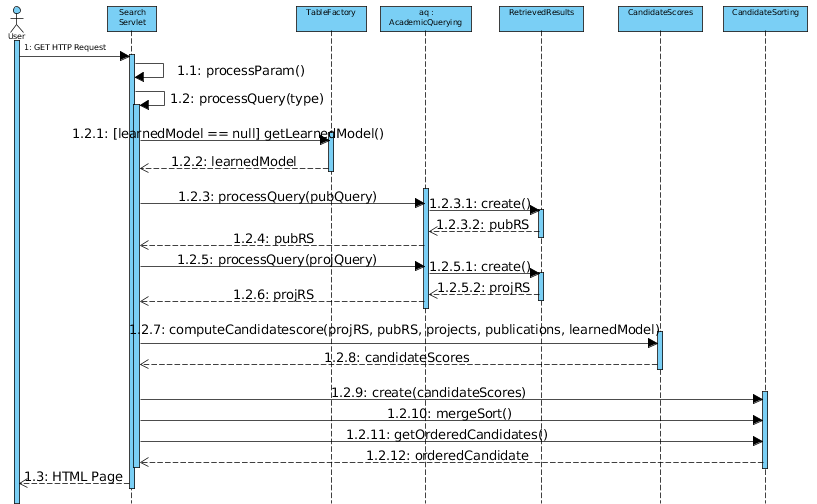
\includegraphics[scale=0.5]{./figures/searchsequence.png}
\caption{Sequence Diagram of Querying} \label{fig:searchsequence} 
\end{figure}

Figure~\ref{fig:searchsequence} illustrates a sequence diagram of querying. This sequence diagram only shows important processes to retrieve
relevant results. Given a query submitted by a user, Search servlet processes parameters sent via GET request by calling processParam() method. This is
followed by invoking processQuery() method which takes one parameter, ``type''. This parameter is used for filter mode. The method processQuery() 
performs tasks discussed in section~\ref{section:union}. There are 2 classes introduced in this section: \textbf{CandidateScores} and 
\textbf{CandidateSorting}. The former is used for computing scores of candidates based on a learned model. The latter
sorts scores of candidates obtained after applying a learned model in descending score as discussed in section~\ref{sec:learnedmodel}.
Figure~\ref{fig:scoreandsorting} shows class diagrams of CandidateScores and CandidateSorting. Important attributes and methods are only shown.

\begin{figure}
\centering
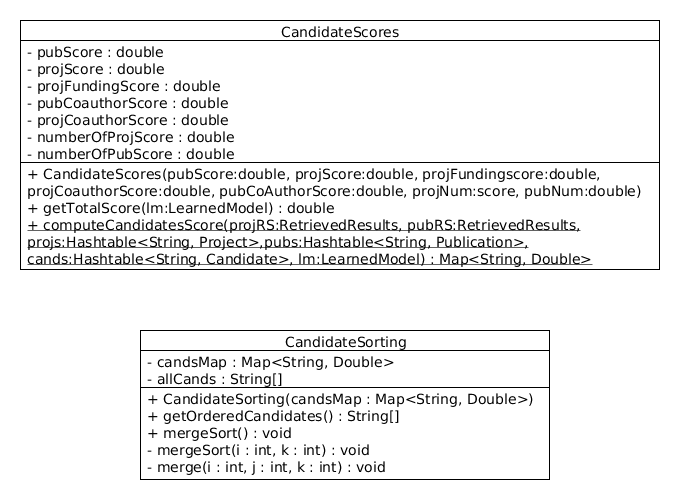
\includegraphics[scale=0.5]{./figures/score&sorting.png}
\caption{Class Diagrams of CandidateScores and CandidateSorting} \label{fig:scoreandsorting} 
\end{figure}




